\documentclass[a4paper,12pt]{article}

\usepackage{graphicx} % Required for inserting images
\usepackage{amsmath,amssymb,amsfonts}
\usepackage{subcaption}
% -----------------------
% Package Imports
% -----------------------

% Set page margins
\usepackage[a4paper, top=1in, bottom=0.8in, left=1.1in, right=0.8in]{geometry}

% Use Times New Roman font
\usepackage{times}

\usepackage{microtype}

\usepackage{array,booktabs,multirow,makecell}
\usepackage{bm}
\usepackage{siunitx}  % For proper unit handling


% Set page margins
\usepackage[a4paper, top=1in, bottom=0.8in, left=1.1in, right=0.8in]{geometry}


% Add page numbering
\pagestyle{plain}

% Enable graphics inclusion
\usepackage{graphicx}
\usepackage{float}
% Enable code listings
\usepackage{listings}
\usepackage{xcolor} % For customizing code colors
\setlength{\parindent}{0pt}
\usepackage{multirow}

\setlength{\parindent}{0pt}
\usepackage{titlesec} % To customize section font size
\titleformat{\section}
{\normalfont\fontsize{14}{16}\bfseries}{\thesection}{1em}{}

\titleformat{\subsection}
{\normalfont\fontsize{14}{16}\bfseries}{\thesubsection}{1em}{}

\begin{document}
	\section{Experiment No. 9}
	
	\section{Experiment Title }
Determination of equivalent Circuit Parameters Using No Load test and Blocked Rotor Test.

	
	\section{Objective}
	
	The objectives of this lab are as follows:
	\begin{itemize}
		\item 	To understand the equivalent-circuit representation of a three-phase induction motor
		\item 	To determine the core losses and magnetizing branch parameters using the no-load test.
		
		\item  To find the stator and referred rotor resistance and leakage reactance using the locked-rotor
		test.
		
		
	\end{itemize}
\section{Theory}

The equivalent-circuit model of a three-phase induction motor provides a simplified representation of its electrical and magnetic behavior. By determining parameters such as stator and rotor resistance, leakage reactance, and magnetizing branch components, the motor's performance can be predicted under various operating conditions.

Two standard tests are commonly performed to obtain these equivalent-circuit parameters:
\begin{itemize}
	\item \textbf{No-Load Test}: Determines core losses and magnetizing branch parameters.
	\item \textbf{Locked Rotor Test}: Determines stator and referred rotor impedance parameters.
\end{itemize}

\subsection{No-Load Test}
The no-load test is conducted with the motor running freely without any mechanical load. The primary goals of this test are to:
\begin{itemize}
	\item Determine the rotational losses (friction, windage, core, and stray losses).
	\item Estimate the magnetizing current and core loss component.
\end{itemize}

During the no-load test, the stator current \( I_1 \), applied voltage \( V_L \), and input power \( P_{\text{in}} \) are measured. The stator copper losses under no-load conditions are calculated as:

\begin{equation}
	P_{\text{SCL}} = 3 I_1^2 R_1
\end{equation}

Hence, the total input power can be expressed as:

\begin{equation}
	P_{\text{in}} = P_{\text{SCL}} + P_{\text{core}} + P_{\text{F\&W}} + P_{\text{misc}} = 3 I_1^2 R_1 + P_{\text{rot}}
\end{equation}

Here, the total rotational losses are:

\begin{equation}
	P_{\text{rot}} = P_{\text{core}} + P_{\text{F\&W}} + P_{\text{misc}}
\end{equation}

By subtracting the stator copper losses from the measured input power, the rotational losses can be determined. Additionally, from the no-load current and power factor angle, the shunt branch parameters \( R_0 \) and \( X_0 \), representing the core loss resistance and magnetizing reactance respectively, can be calculated.

\subsection{Locked Rotor Test}
The locked rotor test is performed with the rotor prevented from rotating. A reduced balanced three-phase voltage is applied to draw rated current. Using the measured values of input voltage, current, and power, the following calculations are made:

\begin{itemize}
	\item Total impedance referred to stator:
	\begin{equation}
		Z_{\text{LR}} = \frac{V_\phi}{I_1} = \frac{V_T}{\sqrt{3} I_L}
	\end{equation}
	
	\item Input power:
	\begin{equation}
		P_{\text{in}} = \sqrt{3} V_T I_L \cos\theta
	\end{equation}
\end{itemize}

From this test, the total resistance and reactance are:

\begin{equation}
	R_{\text{LR}} = R_1 + R_2' = \frac{P_{\text{in}}}{3 I_1^2}
\end{equation}

\begin{equation}
	X_{\text{LR}} = \sqrt{Z_{\text{LR}}^2 - R_{\text{LR}}^2} = X_1 + X_2'
\end{equation}

Since the locked rotor test is usually conducted at low frequency, the reactance is scaled to rated frequency as:

\begin{equation}
	X_{\text{LR (at rated freq)}} = \frac{f_{\text{rated}}}{f_{\text{test}}} \cdot X_{\text{LR (test)}}
\end{equation}

\begin{figure}[h!]
	\centering
%	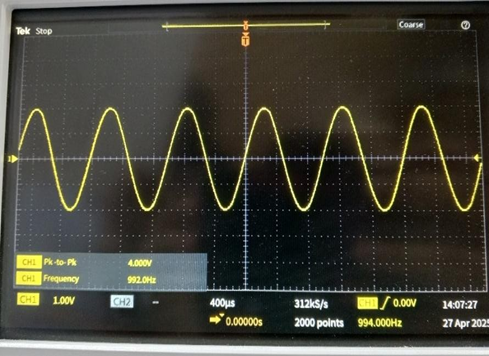
\includegraphics[width=5in,height=2.3in]{9.1}
	\caption*{\textbf{Figure 9.1:} Equivalent Circuit Diagram of Induction Motor}
\end{figure}

\subsection{Equivalent Circuit Parameters}
With the data obtained from the no-load and locked rotor tests, the equivalent circuit parameters can be determined:

\begin{itemize}
	\item Stator resistance \( R_1 \) is measured directly or approximated as half of \( R_{\text{LR}} \).
	\item Referred rotor resistance \( R_2' = R_{\text{LR}} - R_1 \).
	\item Leakage reactance \( X_1 = X_2' = \frac{X_{\text{LR}}}{2} \).
	\item Core-loss and magnetizing branch parameters \( R_0 \) and \( X_0 \) are derived from no-load test data.
\end{itemize}

These parameters provide an accurate representation of the induction motor's internal characteristics and allow for prediction of performance under different load conditions.

	
	\newpage
	
	
	\section{Circuit Diagram}
	\begin{figure}[H]
		\centering

		
	\end{figure}
	
		\begin{figure}[H]
		\centering
		\begin{subfigure}[t]{0.9\textwidth}
			\centering
			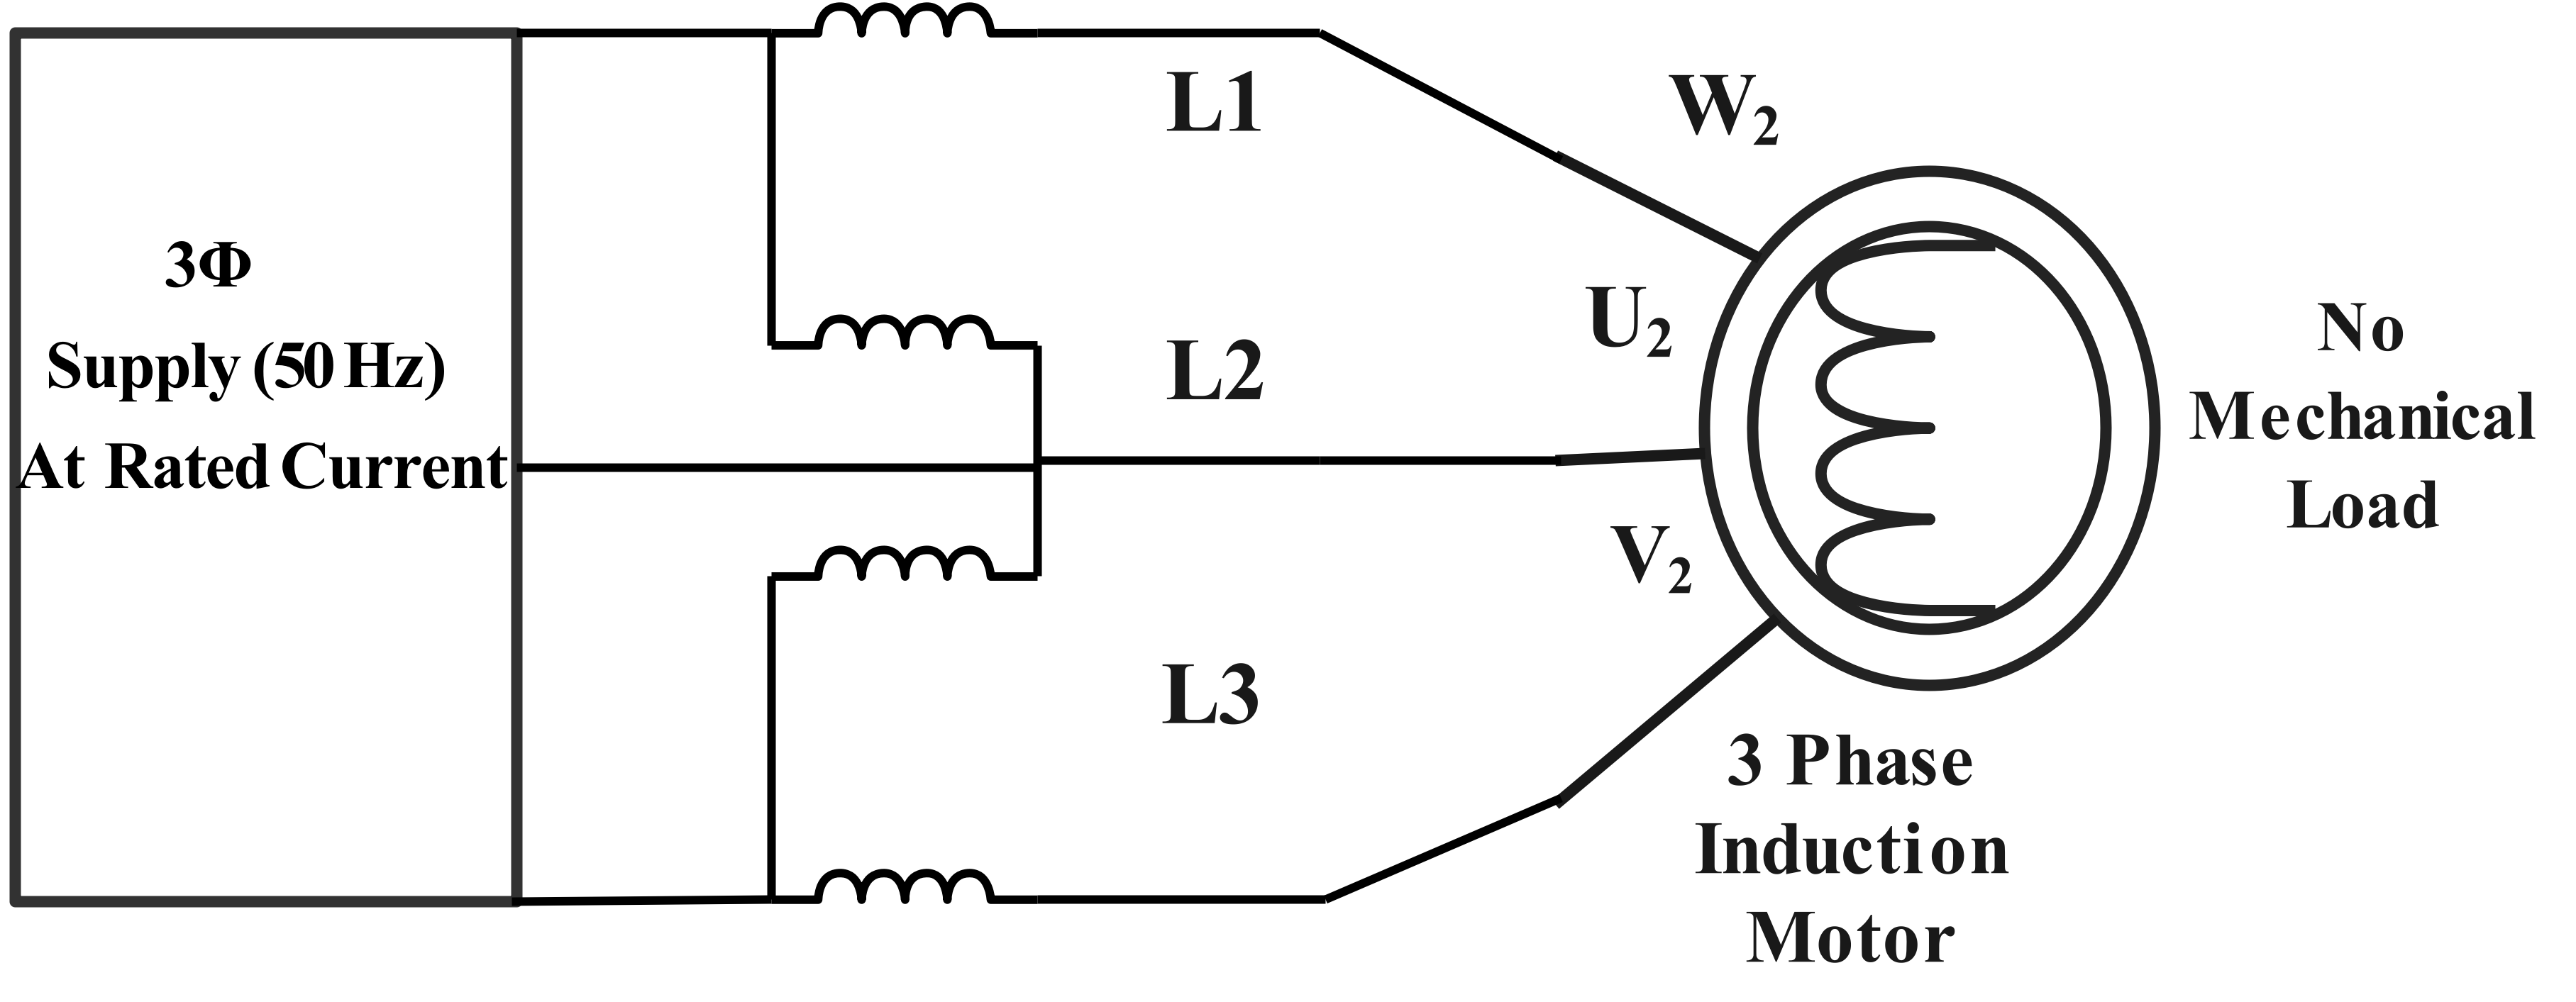
\includegraphics[width=1\textwidth]{Images/2}
			\caption{Test circuit for the no-load test of an induction motor}
			\vspace{0.1cm}
		\end{subfigure}
	
		\begin{subfigure}[t]{0.9\textwidth}
			\centering
			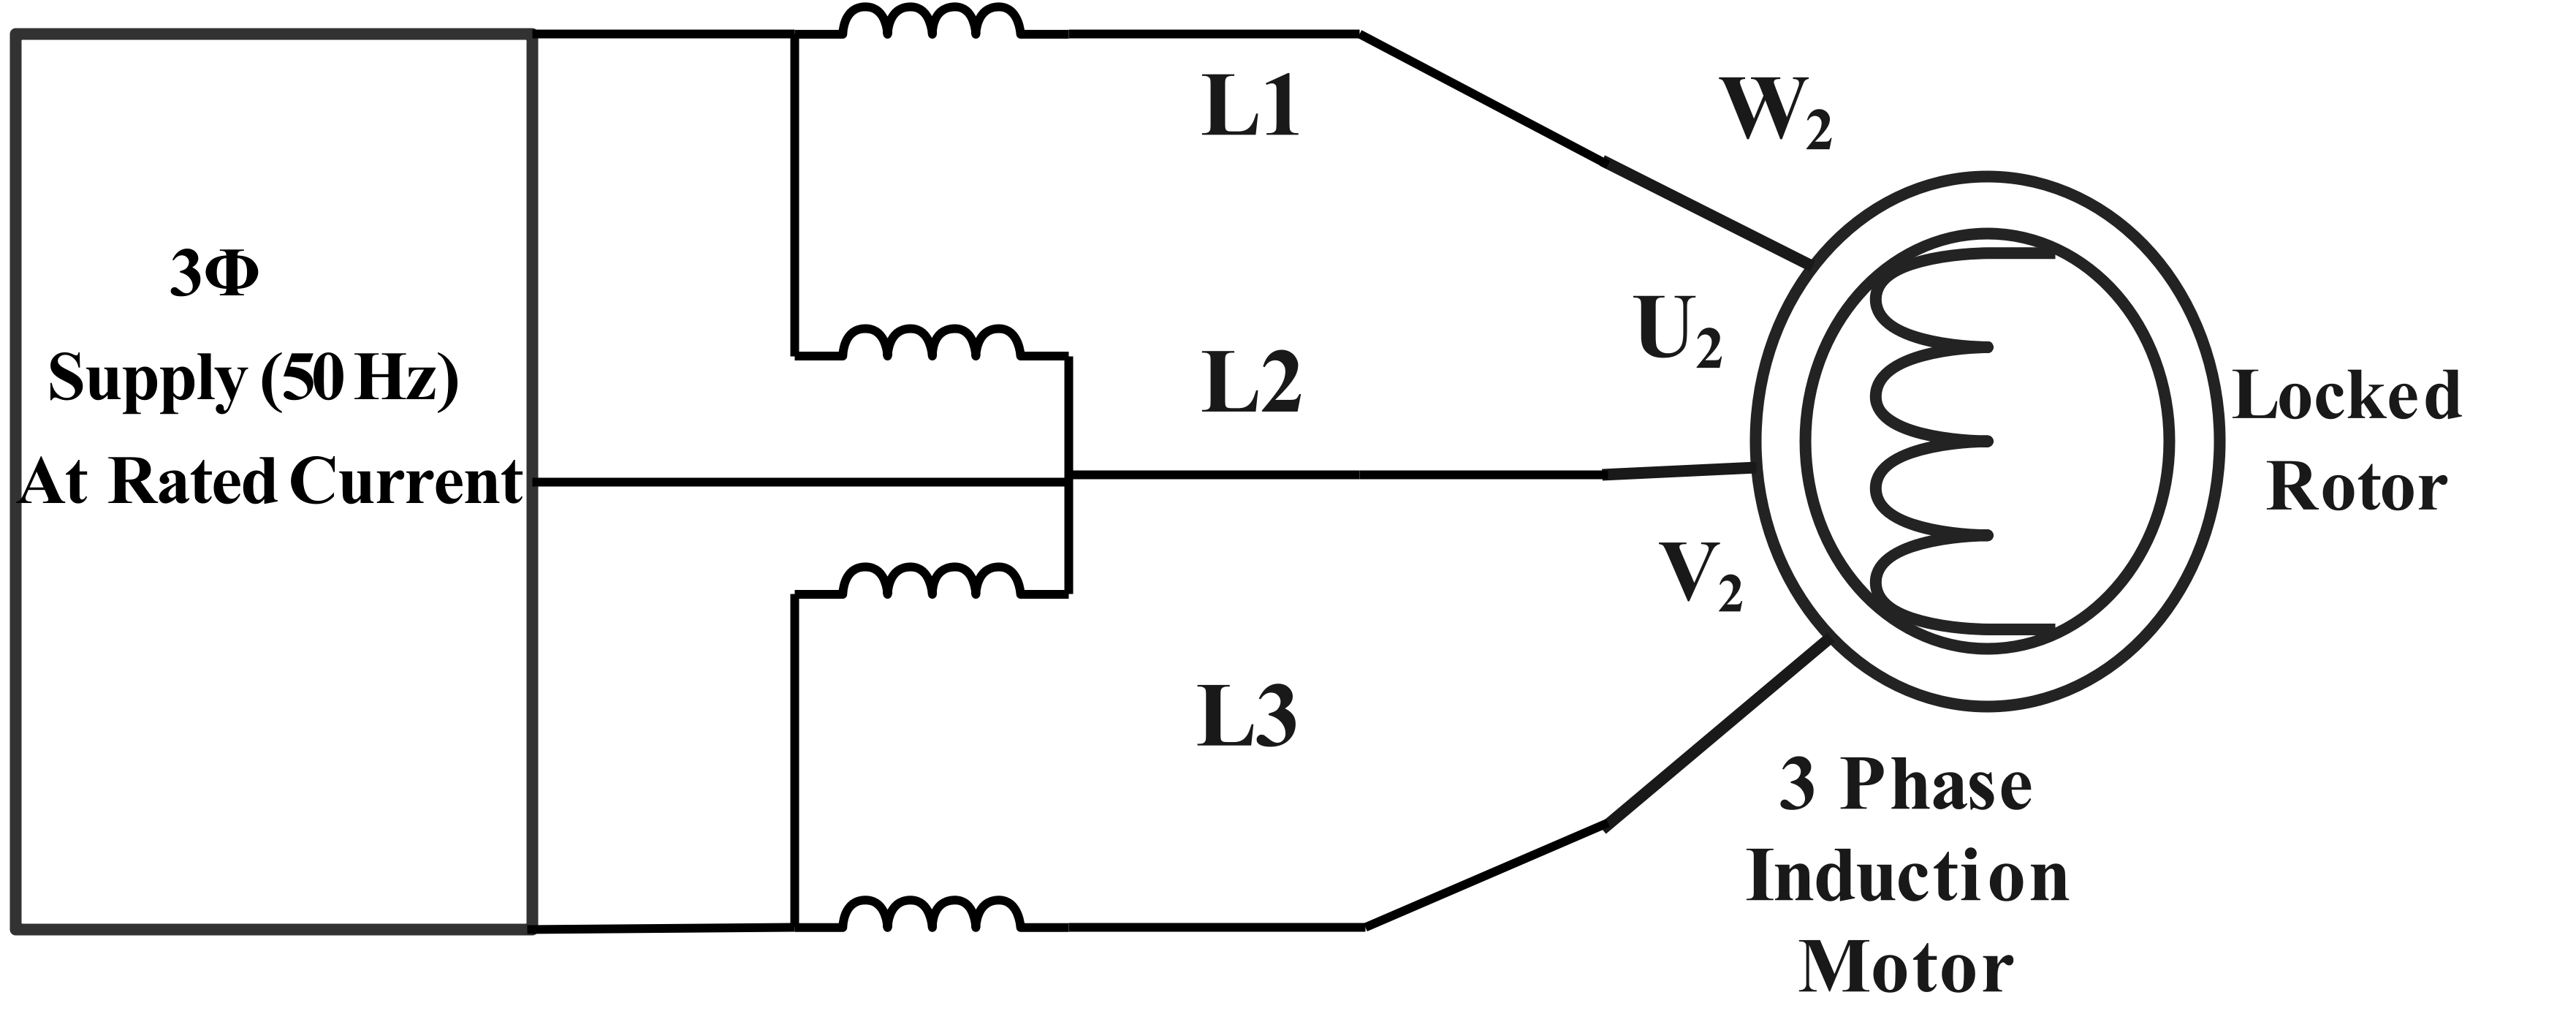
\includegraphics[width=1\textwidth]{Images/1}
			\caption{Test circuit for the mechanical load test of an induction motor}
		\end{subfigure}
	\end{figure}
	
\section{Required Apparatus}

\begin{enumerate}
	\item \textbf{3-Phase Induction Motor}
	\begin{enumerate}
		\item Max Current: $I_{max} = 1.5\, \text{A}$
		\item Max Speed: $Speed_{max} = 3000\, \text{rpm}$
		\item Max Voltage: $V_{max} = 230\, \text{V}$
	\end{enumerate}
	
	\item \textbf{3-Phase AC Meter}
	\begin{enumerate}
		\item Voltage: $500\, \text{V}_{rms}$
		\item Current: $5\, \text{A}$
	\end{enumerate}
	
	\item \textbf{Three-Phase Variable AC Supply}
	\begin{enumerate}
		\item Voltage Range: $0 - 430\, \text{V}$
		\item Current: $3\, \text{A}$
	\end{enumerate}
	
	\item \textbf{Connecting Wires}
\end{enumerate}





\section{Data Table}

\begin{table}[H]
	\centering
	\begin{tabular}{|l|c|c|}
		\hline
		\textbf{Parameter} & \textbf{No Load Test} & \textbf{Locked Rotor Test} \\
		\hline
		Power, $P$ (W) & 13.6 & 45.5 \\
		\hline
		Voltage, $V$ (V) & 400.0 & 76.4  \\
		\hline
		Current, $I$ (A) & 1.32 & 1.501 \\
		\hline
	\end{tabular}
	\caption*{\textbf{Table 9.1:} No Load and Locked Rotor Test Data (Per Phase)}
\end{table}


\section{Calculation}

\subsection*{Locked Rotor Test}
\begin{align*}
	\text{Input Power (per phase)} & : P_{sc} = \SI{45.5}{\watt} \\
	\text{Voltage} & : V_{sc} = \SI{76.4}{\volt} \\
	\text{Current} & : I_{sc} = \SI{1.501}{\ampere} \\
	\text{Power Factor} & : \cos\theta = \frac{P_{sc}}{3V_{sc}I_{sc}} = \frac{45.5}{3 \times 76.4 \times 1.501} = 0.133 \\
	\text{Impedance Magnitude} & : |Z| = \frac{V_{sc}}{I_{sc}} = \frac{76.4}{1.501} = \SI{50.9}{\ohm} \\
	\text{Impedance (Rectangular)} & : Z = |Z|(\cos\theta + j\sin\theta) = 50.9(0.133 + j0.991) \\
	& = \SI{6.77}{\ohm} + j\SI{50.42}{\ohm} \\
	\text{Stator Resistance (approx)} & : R_1 + R_2' = \SI{6.77}{\ohm} \\
	\text{Leakage Reactance (approx)} & : X_1 + X_2' = \SI{50.42}{\ohm}
\end{align*}

\subsection*{No Load Test}
\begin{align*}
	\text{Input Power (per phase)} & : P_{oc} = \SI{13.6}{\watt} \\
	\text{Voltage} & : V_{oc} = \SI{400.0}{\volt} \\
	\text{Current} & : I_{oc} = \SI{1.32}{\ampere} \\
	\text{Power Factor} & : \cos\theta_0 = \frac{P_{oc}}{3V_{oc}I_{oc}} = \frac{13.6}{3 \times 400.0 \times 1.32} = 0.0086 \\
	\text{Reactive Factor} & : \sin\theta_0 = \sqrt{1 - \cos^2\theta_0} = \sqrt{1 - 0.0086^2} = 0.99996 \\
	\text{Magnetizing Current} & : I_m = I_{oc}\sin\theta_0 = 1.32 \times 0.99996 = \SI{1.3199}{\ampere} \\
	\text{Core Loss Current} & : I_c = I_{oc}\cos\theta_0 = 1.32 \times 0.0086 = \SI{0.0114}{\ampere} \\
	\text{Core Loss Resistance} & : R_c = \frac{V_{oc}}{I_c} = \frac{400.0}{0.0114} = \SI{35087.7}{\ohm} \\
	\text{Magnetizing Reactance} & : X_m = \frac{V_{oc}}{I_m} = \frac{400.0}{1.3199} = \SI{303.0}{\ohm}
\end{align*}

\section{Equvalent Circuit Diagram}

\begin{figure}[H]
	\centering
	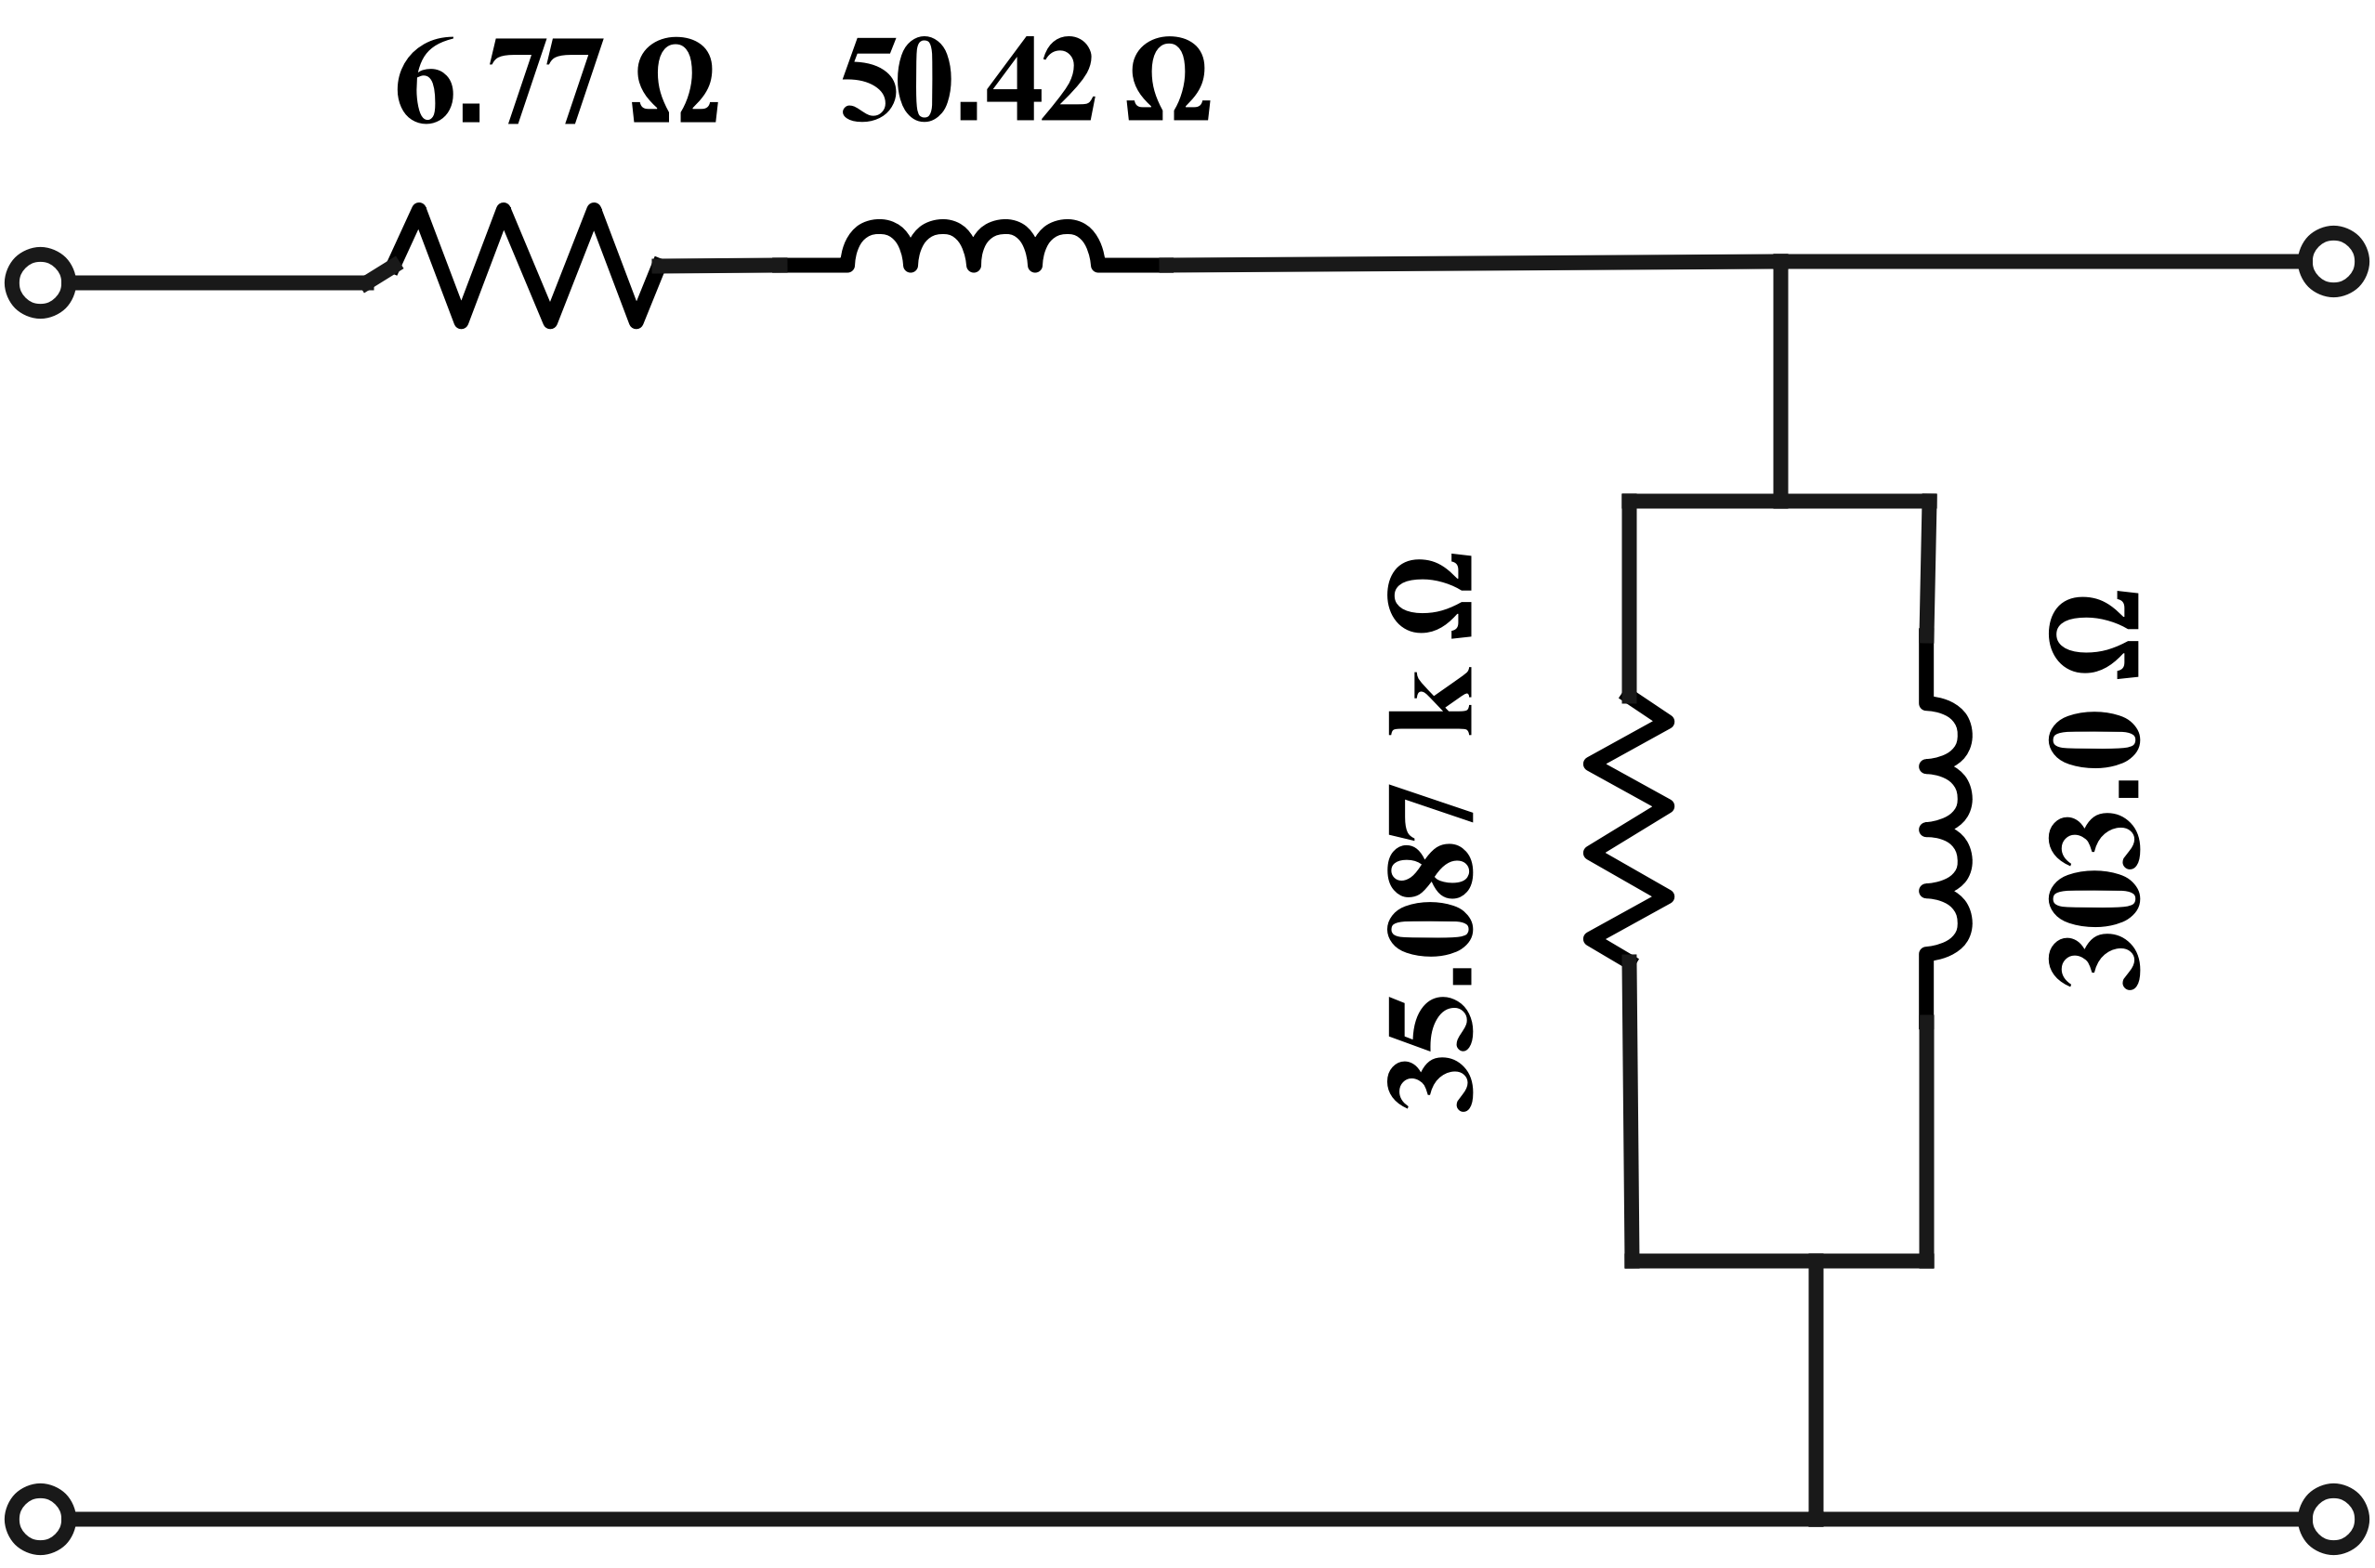
\includegraphics[width=0.6\linewidth]{Images/3}
	\caption{}
	\label{fig:3}
\end{figure}


	
\section{Discussion}

In this experiment, the equivalent circuit parameters of a three-phase induction motor were determined. The no-load test was performed to obtain the magnetizing branch parameters and rotational losses, while the locked-rotor test was conducted to estimate the stator and rotor resistance and leakage reactance. Input power ($P$), current ($I$), and voltage ($V$) were measured in both tests. During the locked-rotor test, the voltage was adjusted to maintain rated current. The calculated parameters matched theoretical expectations and confirmed the effectiveness of this testing method in analyzing motor behavior under varying load conditions.

	
	
	
\end{document}
